\documentclass[10pt]{article}
\usepackage[polish]{babel}
\usepackage[utf8]{inputenc}
\usepackage[T1]{fontenc}
\usepackage{amsmath}
\usepackage{amsfonts}
\usepackage{amssymb}
\usepackage[version=4]{mhchem}
\usepackage{stmaryrd}
\usepackage{graphicx}
\usepackage[export]{adjustbox}
\graphicspath{ {./images/} }

\title{I Konkurs matematyczny St@ś \\
 XIV LO im. Stanisława Staszica \\
 29 maja 2001 roku }

\author{}
\date{}


\begin{document}
\maketitle
\section*{klasa V}
Na rozwiqzanie poniższych zadań masz 90 minut. Kolejność rozwiqzywania tych zadań jest dowolna.\\
Wszystkie zadania sa jednakowo punktowane. Maksymalną liczbę punktów może uzyskać jedynie pelne rozwiazanie, z uzasadnieniem i odpowiedzia.\\
Używanie korektora i korzystanie z kalkulatora jest niedozwolone.

\section*{Zadanie 1.}
Takim samym literom odpowiadają takie same cyfry, a różnym literom - różne cyfry. Znajdź te cyfry, tak aby wszystkie działania w pionie i wszystkie działania w poziomie były prawdziwe.

\begin{center}
\begin{tabular}{ccc}
\(\mathrm{A} \mathrm{A}+\quad \mathrm{D}=\mathrm{BC} \mathrm{F}\) &  \\
\(+\quad+\) & + \\
\(\mathrm{B}+\mathrm{DD}\) & \(=\mathrm{DE}\) \\
\hline
\(\mathrm{BC} \mathrm{C}+\mathrm{EC}=\) & BEC \\
\hline
\end{tabular}
\end{center}

\section*{Zadanie 2.}
Czy jest taka pięciocyfrowa liczba pierwsza, którą można zapisać używając jednokrotnie każdej \(z\) cyfr: 2, 4, 5, 6, 8? Odpowiedź uzasadnij.

\section*{Zadanie 3.}
W pewnym wielokacie wypukłym narysowano wszystkie przekątne, „wychodzace" z jednego wierzchołka. Narysowane przekątne podzieliły ten wielokąt na 200 trójkątów. Ile boków ma ten wielokąt? Odpowiedź uzasadnij.

\section*{Zadanie 4.}
Przeciwprostokątna trójkąta prostokątnego równoramiennego ma 12 cm . Oblicz pole tego trójkąta. Odpowiedź uzasadnij.

\section*{Zadanie 5.}
Na trzech ścianach szeṡcianu narysowano symbole. Przerysuj siatkę tego sześcianu i dorysuj na niej brakujące elementy.\\
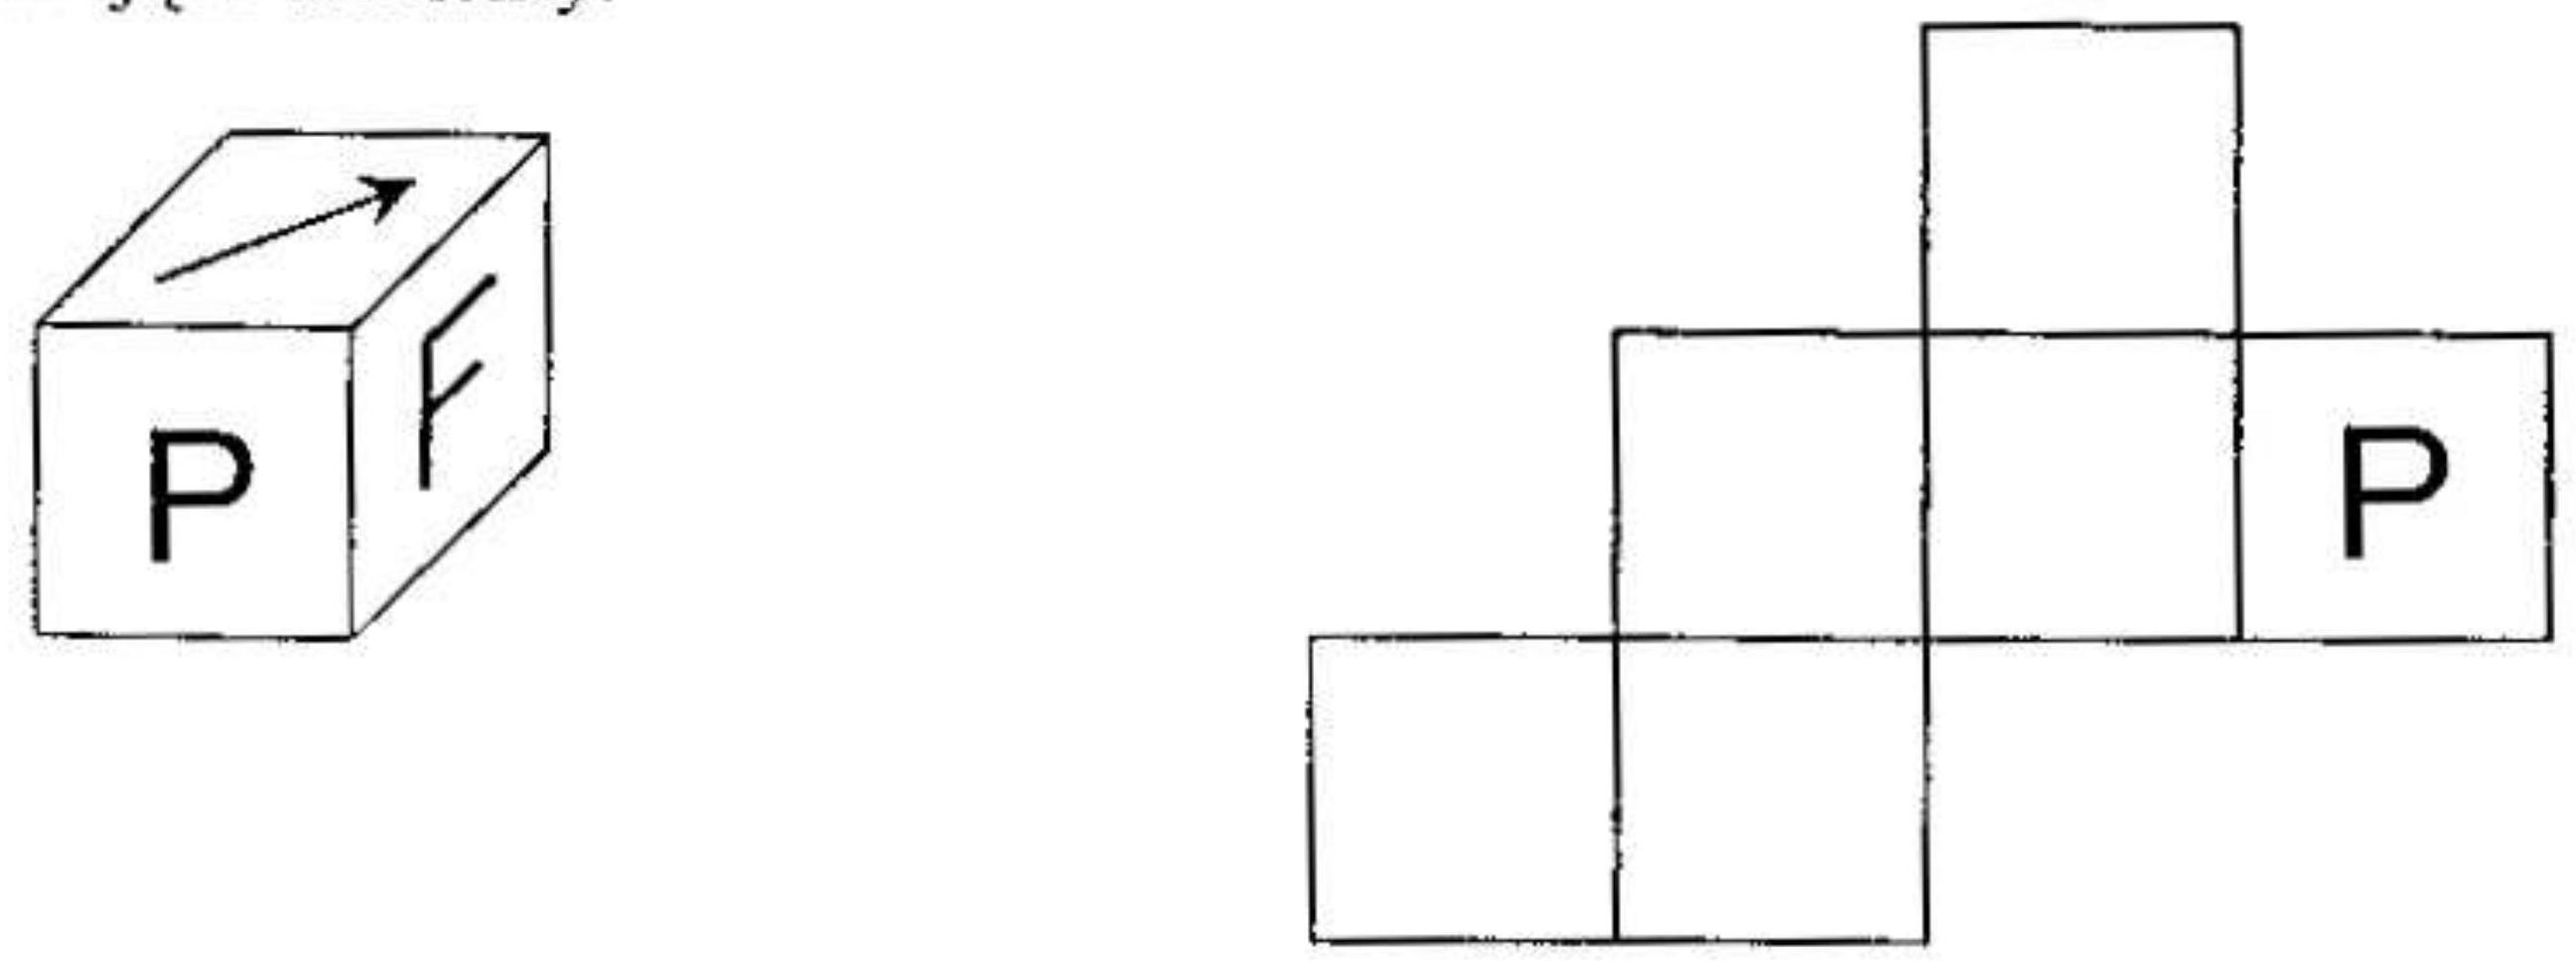
\includegraphics[max width=\textwidth, center]{2024_11_21_deb47e5e36e83c8083c2g-1}


\end{document}